%-----------------------------------------------------------------------
%  Installation de GeOxygene
%

\chapter{Installation de GeOxygene}


%---------------------------------------------------------------------------------
Vous avez maintenant tout ce qu'il faut pour télécharger, gérer, compiler et exécuter GeOxygene.


%---------------------------------------------------------------------------------
\section{Importer le projet GeOxygene}
Dans Eclipse la création d'un nouveau projet s'effectue via l'assistant "nouveau projet". Celui-ci offre en effet une pléthore de modèles. Il suffit donc pour importer GeOxygene de choisir celui qui va extraire un projet Maven depuis un SCM (dans notre cas SVN). 

\medskip

\noindent
Comme décrits dans les deux captures d’écran ci-dessous, cliquer :

\def\imagetop#1{\vtop{\null\hbox{#1}}}
\begin{center}
\begin{tabular}[h]{c|c}        
  {d'abord sur : \emph{File} $\Rightarrow$ \emph{New}  $\Rightarrow$ \emph{Other}}& 
  {puis sur : \emph{Maven}  $\Rightarrow$ \emph{Checkout~Maven~Projects~from~SCM}} \\        
  
  \imagetop{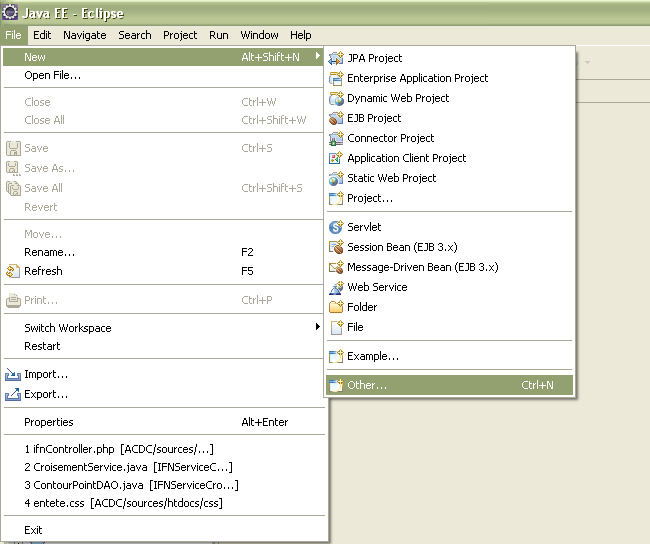
\includegraphics[width=0.39\textwidth]{geoxygeneEtape1}}&
  \imagetop{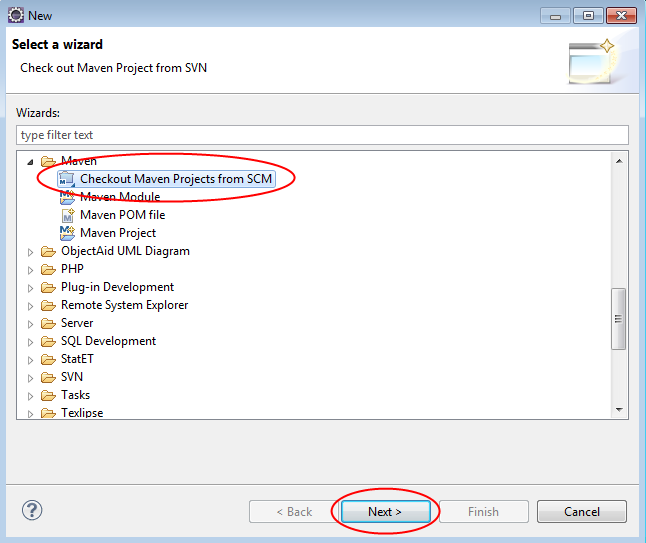
\includegraphics[width=0.61\textwidth]{geoxygeneEtape2}}
\end{tabular}
\end{center}

\newpage

\noindent
Ensuite comme l'indique la figure suivante, sélectionner \emph{svn} dans la première liste comme SCM URL et indiquer l'adresse du svn de GeOxygene~:\\
\begin{itemize}[label=--, leftmargin=* ,parsep=0cm,itemsep=0cm,topsep=0cm]
\item Si vous êtes enregistré sur Sourceforge\footnote{http://sourceforge.net//} et vous avez des droits en tant que développeur ou administrateur sur le projet geoxygene : \\
\href{https://svn.code.sf.net/p/oxygene-project/code/main/trunk/geoxygene}{https://svn.code.sf.net/p/oxygene-project/code/main/trunk/geoxygene}, 
\item Sinon :\\
\href{http://svn.code.sf.net/p/oxygene-project/code/main/trunk/geoxygene/}{http://svn.code.sf.net/p/oxygene-project/code/main/trunk/geoxygene/}, 
\end{itemize}

\begin{center}
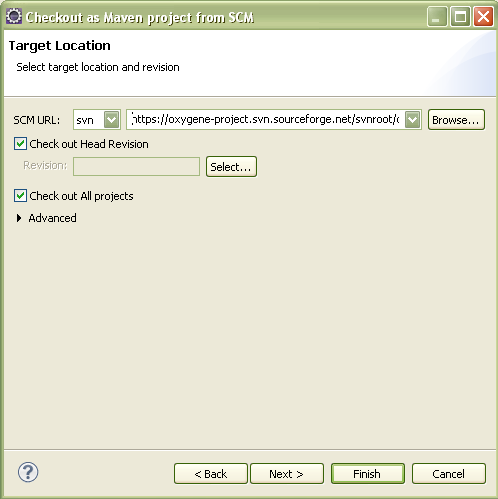
\includegraphics[width=0.5\linewidth]{geoxygeneEtape3}
\end{center}

\bigskip

\noindent
puis cliquer sur "Next".

\bigskip

\noindent
Dans le panneau suivant, vous pouvez:
\begin{itemize}[label=--, leftmargin=* ,parsep=0cm,itemsep=0cm,topsep=0cm]
\item sélectionner le répertoire où sera stocké votre projet (par défaut dans le workspace courant), 
\item ajouter le projet à un working set (c'est à dire un groupe de projets)
\item modifier le nom du (ou des) projet(s) récupéré (s) (dans Advanced). Cette dernière option est utile si vous avez déjà des projets portant des noms identiques ou similaires ou si vous souhaitez ajouter à tous les projets récupérés un préfixe, un suffixe, ou utiliser un template de nom comme [groupId].[artifactId]-[version] qui vous créera, pour geoxygene, un projet nommé \emph{fr.ign.cogit.geoxygene-1.5}.
\end{itemize}

\begin{center}
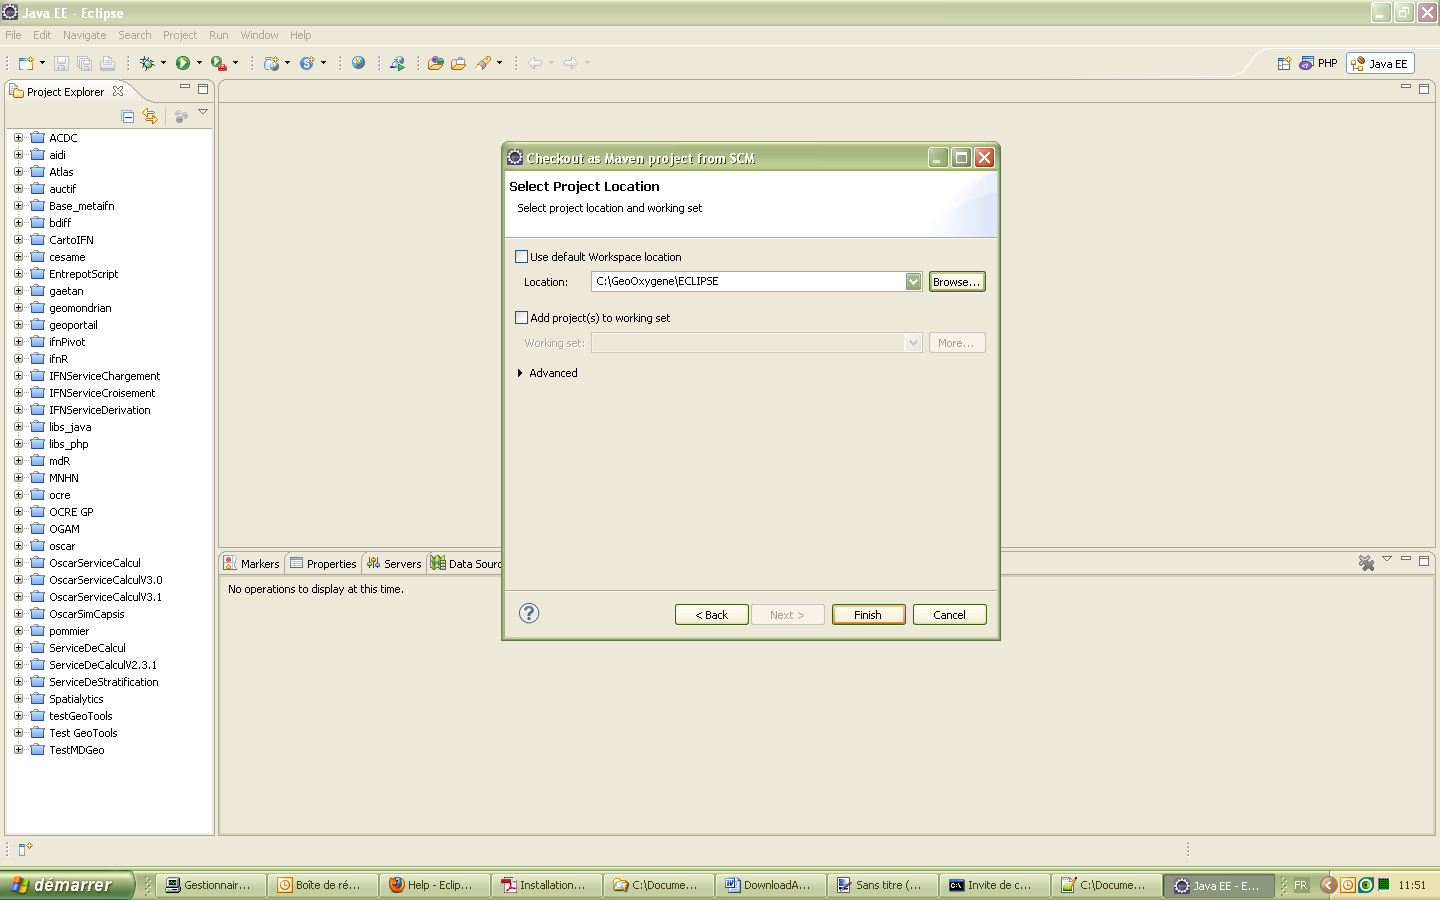
\includegraphics[width=0.5\linewidth]{geoxygeneEtape4}
\end{center}

\bigskip

\noindent
Cliquez ensuite sur Finish.


%---------------------------------------------------------------------------------
\newpage
\section{Compilation}

%-------- cas 1
\begin{flushleft}
    \bf
    1er cas : vous utilisez l'option de compilation automatique
\end{flushleft}

\begin{center}
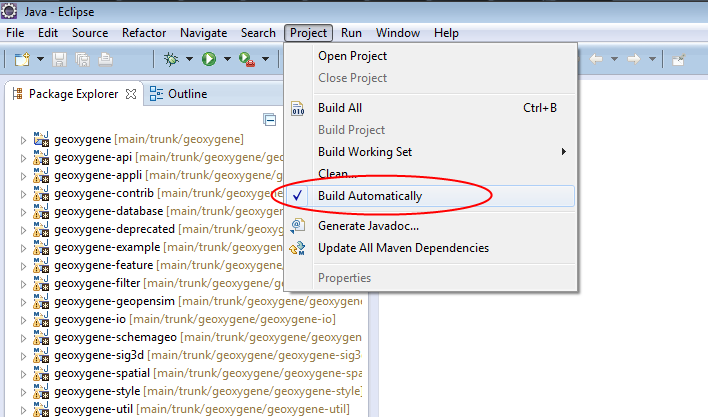
\includegraphics[width=0.5\linewidth]{geoxygeneBuildAutomatically}
\end{center}

\noindent
Vous n'avez rien à faire, la compilation se lance automatiquement

%\begin{center}
%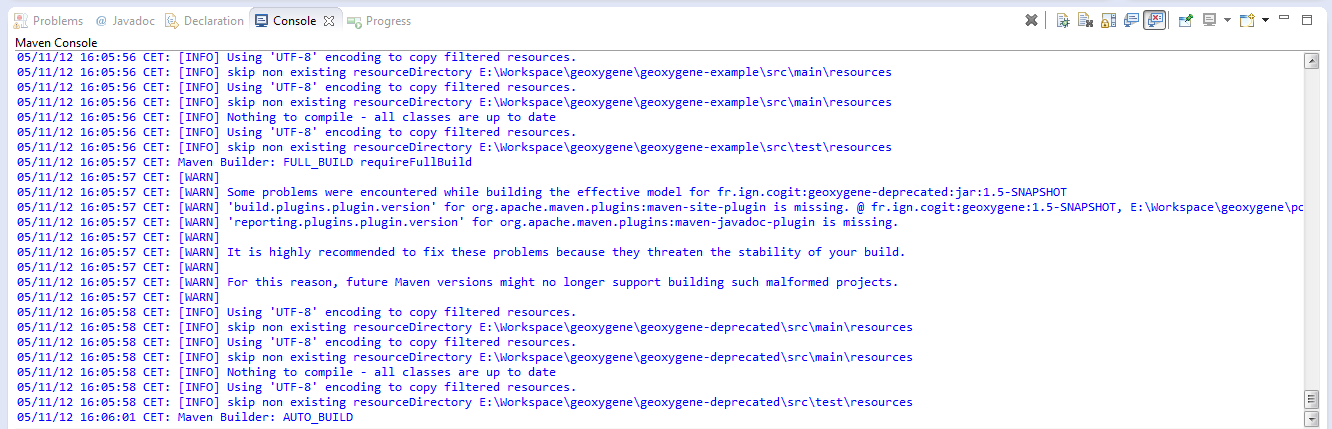
\includegraphics[width=0.5\linewidth]{geoxygeneAutoBuild}
%\end{center}

\smallskip
 
%-------- cas 2
\begin{flushleft}
    \bf
    2ème cas : lancer un maven build manuellement.
\end{flushleft}

\noindent
Pour cela :\\

% 3 tableaux pour les 3 étapes
\begin{tabular}{p{6cm}l}
  {1. Sélectionner dans l'explorateur à droite, le projet "geoxygene". Puis dans le menu, cliquer sur Run $\Rightarrow$ Run Configurations.}&
   \imagetop{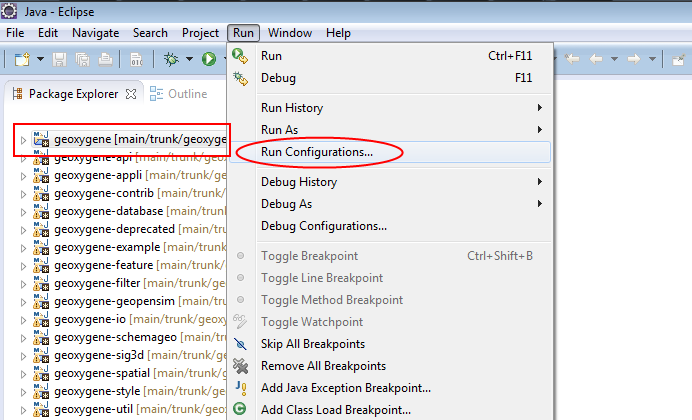
\includegraphics[width=0.45\textwidth]{geoxygeneRunEtape1}} \\
\end{tabular}


\begin{tabular}{p{6cm}l}
   {2.  Sélectionner comme type de run "Maven", puis cliquer dans le menu en haut sur "New launch configuration"}&
   \imagetop{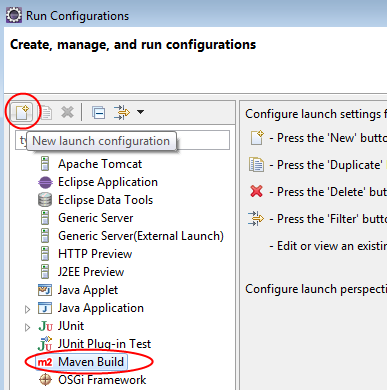
\includegraphics[width=0.4\textwidth]{geoxygeneRunEtape2}} \\
\end{tabular}

\bigskip

\begin{tabular}{p{6cm}l}
   {3.  Dans la nouvelle fenêtre "Run configuration" configurer :
         \begin{enumerate}
         \item \emph{Name} : geoxygene
         \item \emph{Base directory} : saisir le chemin d'installation de GeOxygene (c'est celui de votre Workspace auquel il faut ajouter geoxygene)
         \item \emph{Goal} : clean install. Vous définissez la phase du cycle (clean, install, package, compile, test, site, ...)
         \item d'autres options peuvent être configurées dans cette interface si vous le souhaitez.
         \end{enumerate}}&
   \imagetop{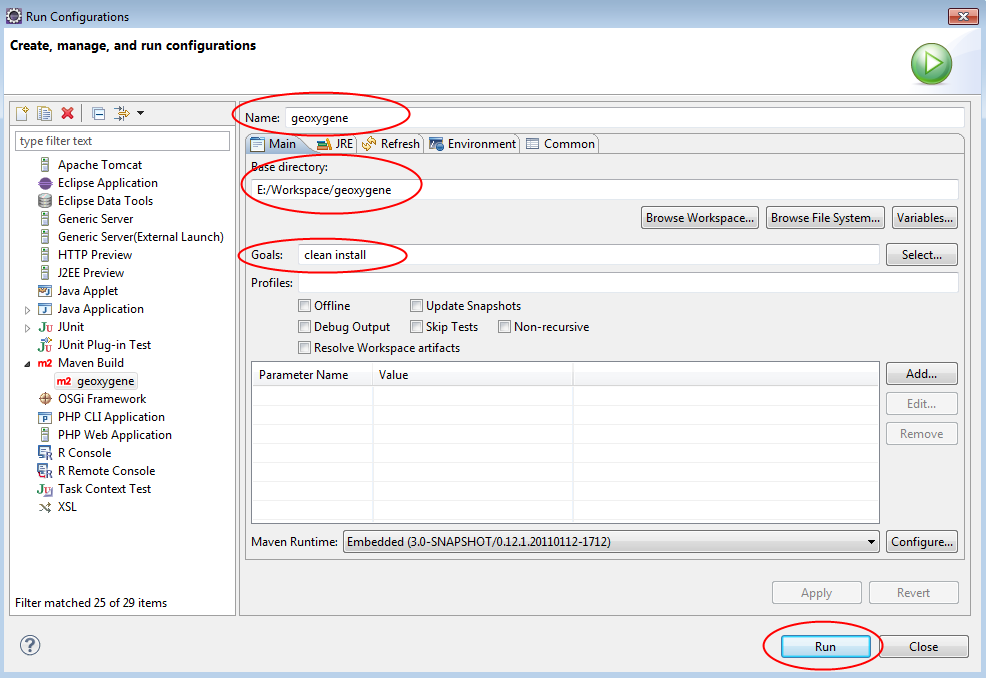
\includegraphics[width=0.55\textwidth]{geoxygeneRunEtape3}} \\
 \end{tabular}





\bigskip
\noindent
Si tout se passe bien, Maven devrait récupérer tous les jars nécessaires et compiler le projet. 

%---------------------------------------------------------------------------------
\section{Exécution d'un exemple}
Une application exemple peut \^etre exécutée~: \emph{fr.ign.cogit.geoxygene.appli.GeOxygeneApplication}.

\bigskip

\noindent
Pour cela ouvrir le fichier GeOxygeneApplication.java qui se trouve dans le module : \\
\begin{tabular}[!t]{llll}
   geoxygene-appli $\Rightarrow$ src/main/java $\Rightarrow$  fr.ign.cogit.geoxygene $\Rightarrow$ appli
\end{tabular}

\bigskip

\noindent
Dans la fenêtre de l'éditeur de la classe, faire un click droit de la souris. Puis cliquer sur :\\
\begin{tabular}[!t]{llll}
"Run As" $\Rightarrow$ "Java Application"
\end{tabular}\\

\begin{center}
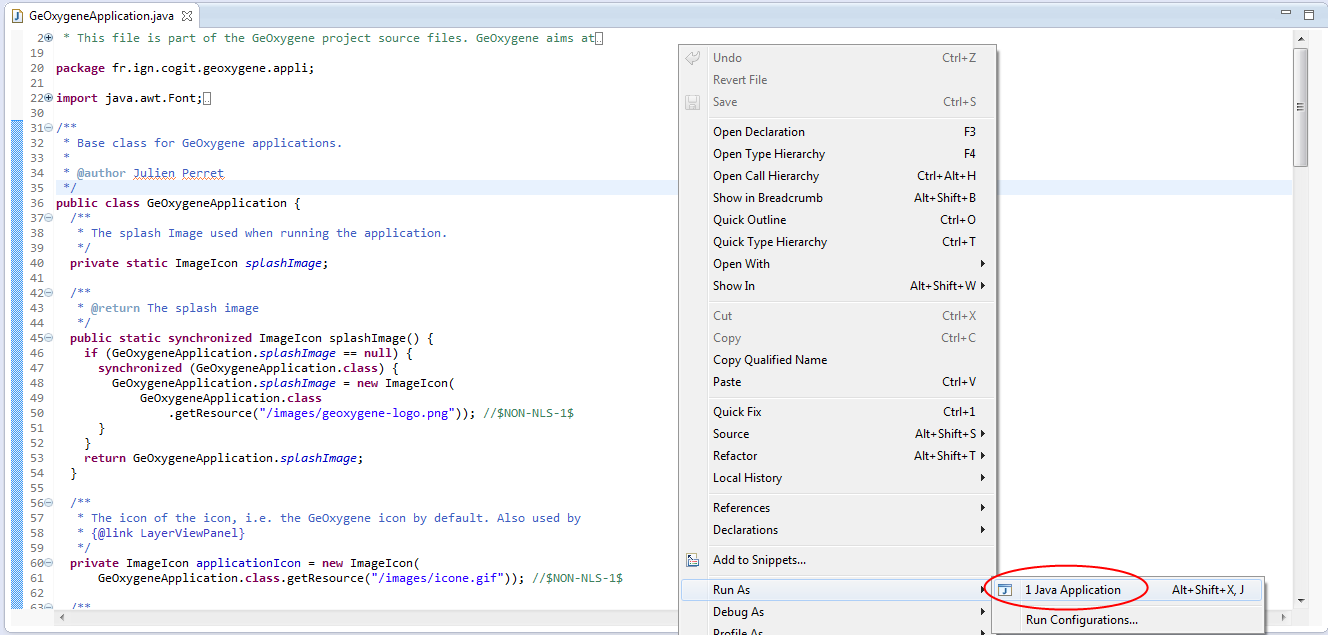
\includegraphics[width=0.5\linewidth]{GeOxygeneAppliRunAs}
\end{center}

L'interface de GeOxygene est lancée !


%---------------------------------------------------------------------------------
\section{Configuration}


%-----
%\subsection{Activation de la console Maven}

%Ouvrir la fenêtre de la console en cliquant sur : {\emph{Window} $\Rightarrow$ \emph{Show View}  $\Rightarrow$ \emph{Console}}. Puis cliquer sur la petite flèche complètement à droite de la fenêtre "Open Console" et sélectionner "Maven Console" comme indiqué ci-dessous :

%\begin{center}
%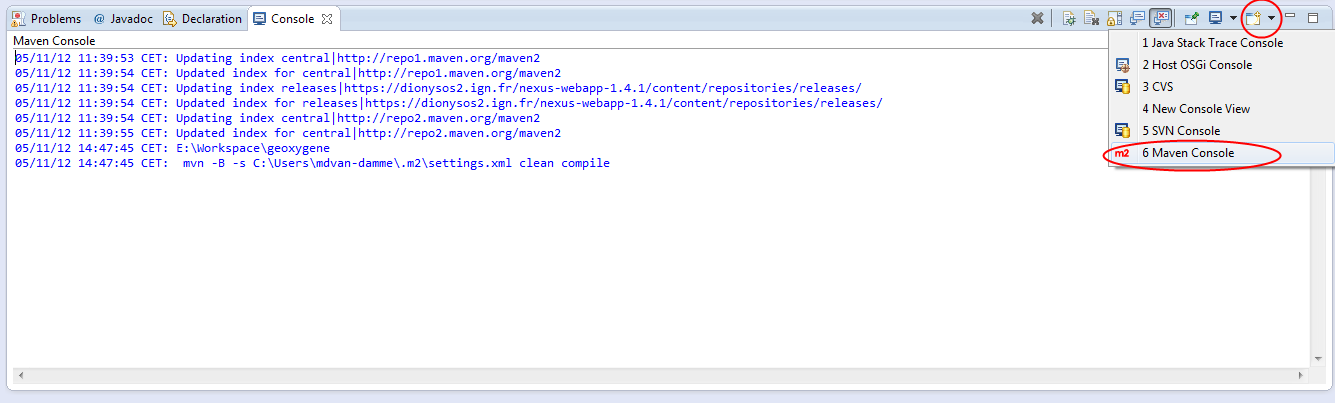
\includegraphics[width=0.5\linewidth]{geoxygeneEtape5}
%\end{center}

%Il peut être utile de travailler avec la sortie de débogage Maven pour diagnostiquer les problèmes.




%---
\subsection{Convention de codage}

Parce qu'on passe plus de temps à lire du code qu’à en écrire, il faut configurer dans Eclipse la convention de programmation adoptée dans GeOxygène. Elle s'inspire avant tout de la convention de programmation recommandée pour tous les développements JAVA. Cette norme est dérivée de celle proposée par SUN à l’adresse :

\begin{tabular}[!t]{llll}
{\href{http://www.oracle.com/technetwork/java/codeconvtoc-136057.html}{http://www.oracle.com/technetwork/java/codeconvtoc-136057.html}}  
\end{tabular}

\noindent
Aller dans "Preferences $\Rightarrow$ Java $\Rightarrow$ Code Style $\Rightarrow$ Formatter" et cliquer sur "Import". 

\begin{center}
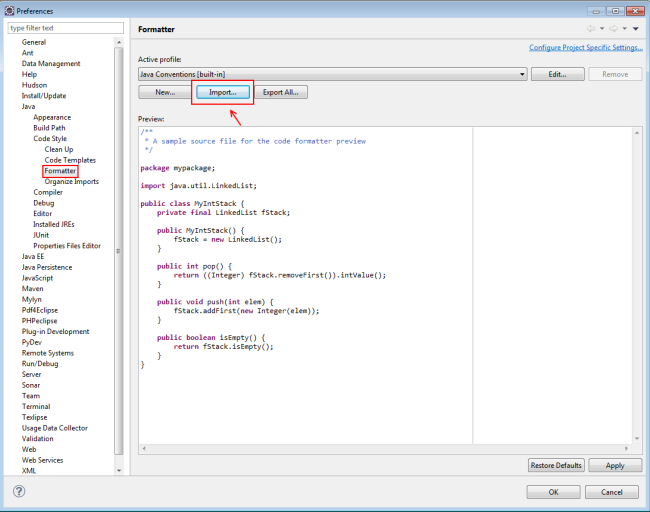
\includegraphics[width=0.5\linewidth]{ConfigEclipseConventionCodage_1}
\end{center}

\noindent
Le template de la convention de nommage du COGIT «java\_cogit\_formatting\_conventions\_v1.xml» se trouve dans le code source du projet GeOxygene :

\begin{tabular}[!t]{llll}
geoxygene $\Rightarrow$  src $\Rightarrow$  main $\Rightarrow$  resources $\Rightarrow$  java\_cogit\_formatting\_conventions\_v1.xml
\end{tabular}

\smallskip

\noindent
Importer ce fichier et choisissez comme "Active profile" : "Java COGIT Formatting Conventions v1" 

\begin{center}
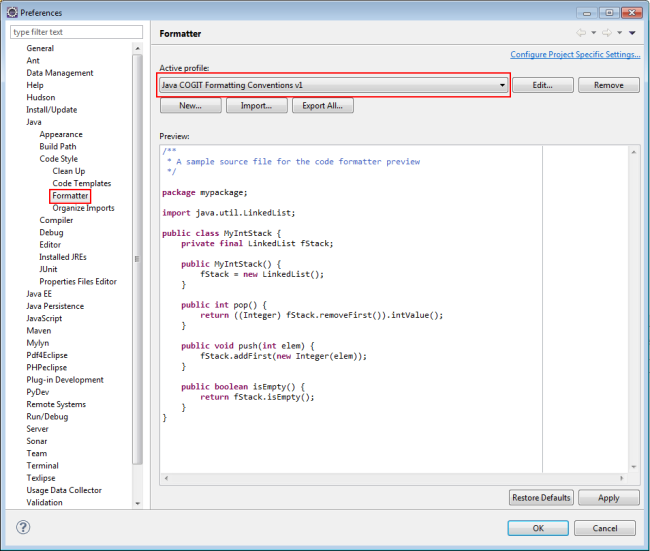
\includegraphics[width=0.5\linewidth]{ConfigEclipseConventionCodage_2}
\end{center}



%\subsection{ Accès aux bases de données}
%\subsection{Journalisation}


